\documentclass[preview]{standalone}

\usepackage{amsmath}
\usepackage{amssymb}
\usepackage{bettelini}
\usepackage{stellar}
\usepackage[version=4]{mhchem}

\hypersetup{
    colorlinks=true,
    linkcolor=black,
    urlcolor=blue,
    pdftitle={Chimica},
    pdfpagemode=FullScreen,
}

\begin{document}

\title{Chimica}
\id{chimica-entalpia}
\genpage

\section{Sviluppo del calore nelle reazioni}

%\begin{snippet}{legami-energia}
%    La rottura di un legame necessita di energia, mentre
%    la formazione di legami libera energia.
%
%    \begin{center}
%    \begin{figure}[h]
%        \centering
%        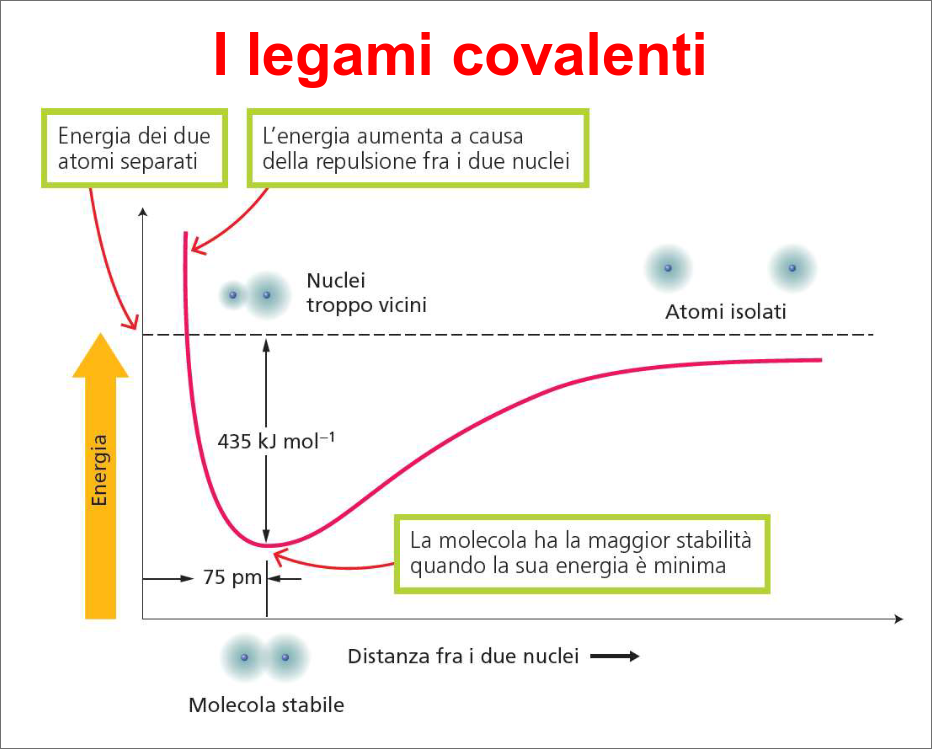
\includegraphics[width=\textwidth]{./cov_bond_energy.png}
%    \end{figure}
%    \end{center}
%\end{snippet}

\end{document}
